\section{Meilenstein 1 $-$ Datenzugriffsschicht}

% Teilaufgabe 1 {{{
\subsection{Teilaufgabe 1: Ausschnitt aus Logischem DM mit Entities und Value Objects}

\subsubsection{Klassendiagramm}
\begin{center}
\begin{tikzpicture}

% Ebene 0 {{{
  \UMLClassAlterName
    {0}
    {0}
    {
      \textbf{Gericht}
        \nodepart{second}
      Name: String \\
      Details: String \\
      Preis: double
    }
    {gericht}
    {minimum width=6cm,text width=2.75cm}

  \UMLClassRelativeToAlterName
    {right=3 of gericht}
    {\textbf{Zutat}\nodepart{second}Name: String}
    {zutat}
    {minimum width=6cm}
% }}}

% Ebene -1 {{{
  \UMLClassRelativeToAlterName
    {below=3 of gericht}
    {\textbf{Speise}\nodepart{second}Name: String}
    {speise}
    {minimum width=6cm}
% }}}

% Ebene -2 {{{
  \UMLClassRelativeToAlterName
    {below=3 of speise}
    {
      \textbf{Zubereitungsanleitung}
        \nodepart{second}
      Anleitung: String
    }
    {za}
    {minimum width=6cm,fill=red!25}

  \UMLClassRelativeToAlterName
    {right=3 of za}
    {\textbf{Zutatenangabe}\nodepart{second}Menge: int}
    {zutatenangabe}
    {minimum width=6cm,fill=red!25}
% }}}

% Verbindungen {{{
  % gericht -- speise {{{
  \draw[umlaggreg-] (gericht.south) -- (speise.north);
  \node[below left=.25 of gericht.south] {*};
  \node[above left=.25 of speise.north] {*};
  \node[left] at ($(gericht)!.5!(speise)$) {Teil von};
  % }}}
  % speise -- za {{{
  \draw[umlcompo-] (speise.south) -- (za.north);
  \node[below left=.25 of speise.south] {1};
  \node[above left=.25 of za.north] {1};
  \node[left] at ($(speise)!.5!(za)$) {beschreibt};
  % }}}
  % zutatenangabe -- za {{{
  \draw[-umlcompo] (zutatenangabe.west) -- (za.east);
  \node[above left=.25 of zutatenangabe.west] {1..*};
  \node[above right=.25 of za.east] {1};
  \node[below] at ($(zutatenangabe)!.5!(za)$) {ben\"otigt};
  % }}}
  % zutatenangabe -- zutat {{{
  \draw (zutatenangabe.north) -- (zutat.south);
  \node[above left=.25 of zutatenangabe.north] {*};
  \node[below left=.25 of zutat.south] {1};
  \node[left] at ($(zutatenangabe)!.5!(zutat)$) {ben\"otigt};
  % }}}
% }}}
\end{tikzpicture}
\end{center}


\subsubsection{Fachliches Glossar}
\begin{tabu} to \linewidth {X|X|X}
% Headerzeile {{{
\hline
\rowcolor{codebordercolor}
Gesch\"aftsobjekt &Attribut &Erkl\"arung \\
% }}}
% Gericht {{{
\hline
Gericht & &Vom Restaurant angebotenes Mahl. \\
  % Name {{{
  \hline
  &Name &Gerichtsbezeichnung. \\
  % }}}
  % Details {{{
  \hline
  &Details &Wird dem Gast angezeigt. Enth\"alt n\"ahere Angaben zu den Zutaten. \\
  % }}}
  % Preis {{{
  \hline
  &Preis &Geldbetrag der f\"ur das Gericht zu bezahlen ist. \\
  % }}}
% }}}
% Speise {{{
\hline
Speise & &Teil eines Gerichts. Beispielsweise w\"are eine Salatbeilage als Speise zu verstehen. \\
  % Name {{{
  \hline
  &Name &Bezeichnung der Speise. \\
  % }}}
% }}}
% Zubereitungsanleitung {{{
\hline
Zubereitungsanleitung & &Leitfaden zur Zubereitung einer Speise. \\
  % Anleitung {{{
  \hline
  &Anleitung &Erkl\"arender Text, der beschreibt, wie eine Speise zuzubereiten ist. \\
  % }}}
% }}}
% Zutat {{{
\hline
Zutat & &Ben\"otigt f\"ur die Zubereitung einer Speise. \\
  % Name {{{
  \hline
  &Name &Bezeichnung der Zutat. \\
  % }}}
% }}}
% Zutatenangabe {{{
\hline
Zutatenangabe & &Zuordnung zwischen Zutat und Zubereitungsanleitung.
                 Gibt die Menge einer Zutat an, die f\"ur die Zubereitung notwendig ist. \\
  % Menge {{{
  \hline
  &Menge &Die ben\"otigte Menge. \\
  % }}}
% }}}
\hline
\end{tabu}


\subsubsection{Erweiterungen der Aufgabenstellung}

Da es in unserem Logischen Datenmodell keine 1:1-Beziehung gab,
haben wir eine zus\"atzliche redundante Entit\"at eingebaut.

Hierbei handelt es sich um die Entit\"at Speise. Diese Entit\"at
h\"atte genauso gut einfach Teil der Zubereitungsanleitung sein
k\"onnen und ist nur in unser Modell aufgenommen worden, damit
wir die f\"ur die Aufgabenstellung ben\"otigte 1:1-Beziehung in
unserem Diagramm haben.

\subsubsection{Erl\"auterungen}

Wir haben Zubereitungsanleitung als Value Object und nicht als
Entity deklariert, da hier unserer Meinung nach Sharing nicht
sinnvoll ist und ein Zubereitungsanleitungsobjekt deshalb
persistent als Teil der zugeordneten Speise in der Datenbank
gespeichert werden sollte.

Gleiches gilt f\"ur die Zutatenmenge.

% }}}

\newpage

% Teilaufgabe 2 {{{
\subsection{Teilaufgabe 2: Entities und Value Objects mit JPA-Annotierung}

\subsubsection{Annotationen der Entities und Value Objects}
% Gericht {{{
\begin{mdframed}[style=codebox]
\textbf{Gericht}
\lstinputlisting[language=Java, firstline=16, lastline=31]
{../code/ms1JPASpringDemo/src/main/java/ms1jpaspringdemo/entities/Gericht.java}
\end{mdframed}
% }}}
% Speise {{{
\begin{mdframed}[style=codebox]
\textbf{Speise}
\lstinputlisting[language=Java, firstline=8, lastline=18]
{../code/ms1JPASpringDemo/src/main/java/ms1jpaspringdemo/entities/Speise.java}
\end{mdframed}
% }}}
% Zubereitungsanleitung {{{
\begin{mdframed}[style=codebox]
\textbf{Zubereitungsanleitung}
\lstinputlisting[language=Java, firstline=13, lastline=20]
{../code/ms1JPASpringDemo/src/main/java/ms1jpaspringdemo/entities/Zubereitungsanleitung.java}
\end{mdframed}
% }}}
% Zutat {{{
\begin{mdframed}[style=codebox]
\textbf{Zutat}
\lstinputlisting[language=Java, firstline=9, lastline=14]
{../code/ms1JPASpringDemo/src/main/java/ms1jpaspringdemo/entities/Zutat.java}
\end{mdframed}
% }}}
% Zutatenangabe {{{
\begin{mdframed}[style=codebox]
\textbf{Zutatenmenge}
\lstinputlisting[language=Java, firstline=5, lastline=10]
{../code/ms1JPASpringDemo/src/main/java/ms1jpaspringdemo/entities/Zutatenmenge.java}
\end{mdframed}
% }}}


% H2-Console {{{
\subsubsection{H2-Console}

% Gerichtstabelle {{{
\begin{figure}[H]
\centering
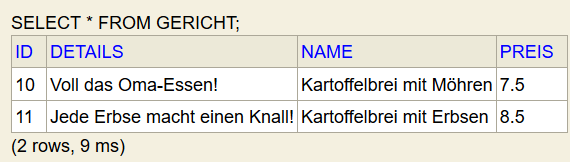
\includegraphics{ms1/screenshots/gericht_table.PNG}
\caption{Gerichtstabelle}
\end{figure}
% }}}

% Speisentabelle {{{
\begin{figure}[H]
\centering
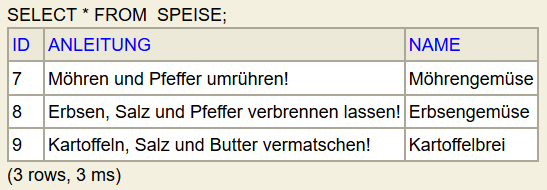
\includegraphics{ms1/screenshots/speise_tbl.PNG}
\caption{Speisentabelle}
\end{figure}
% }}}

% Zutatentabelle {{{
\begin{figure}[H]
\centering
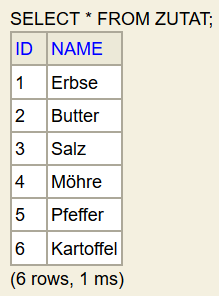
\includegraphics{ms1/screenshots/zutat_tbl.PNG}
\caption{Zutatentabelle}
\end{figure}
% }}}

% Zutatenmengentabelle {{{
\begin{figure}[H]
\centering
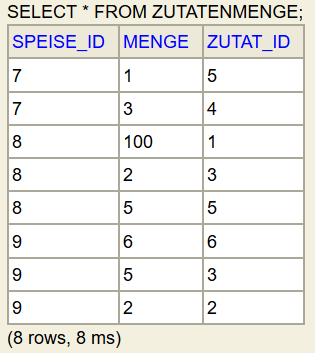
\includegraphics{ms1/screenshots/zutatenmenge_tbl.PNG}
\caption{Zutatenmengentabelle}
\end{figure}
% }}}

% Zuordnungstabelle Gericht - Speise {{{
\begin{figure}[H]
\centering
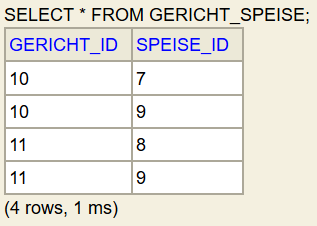
\includegraphics{ms1/screenshots/gericht_speise_tbl.PNG}
\caption{Zuordnungstabelle Gericht - Speise}
\end{figure}
% }}}
% }}}
% }}}

% Teilaufgabe 3 {{{
\subsection{Teilaufgabe 3: Factories und Repositories}

% Gericht Factory {{{
\begin{mdframed}[style=codebox]
\textbf{Factory für Erstellung von Gerichten}
\lstinputlisting[language=Java, firstline=11, lastline=34]
{../code/ms1JPASpringDemo/src/main/java/ms1jpaspringdemo/factories/GerichtFactory.java}
\end{mdframed}
% }}}

Hier sieht man gut warum Factories notwendig sind. 
Bei der Estellung von Gerichten muss zugleich die R\"uckreferenz von 
Speise auf Gericht gesetzt werden.

% Speise Repository {{{
\begin{mdframed}[style=codebox]
\textbf{Factory für Erstellung von Gerichten}
\lstinputlisting[language=Java, firstline=12, lastline=17]
{../code/ms1JPASpringDemo/src/main/java/ms1jpaspringdemo/repositories/SpeiseRepository.java}
\end{mdframed}
%}}}

% Aufruf Query {{{
\begin{mdframed}[style=codebox]
\textbf{Ausgabe in der Konsole}
\lstinputlisting[language=Java, firstline=103, lastline=105]
{../code/ms1JPASpringDemo/src/main/java/ms1jpaspringdemo/SampleData.java}
\end{mdframed}
%}}}

Folgendes wird dann in der Konsole ausgegeben:

% Ausgabe Konsole{{{
\begin{figure}[H]
\centering
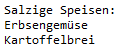
\includegraphics{ms1/screenshots/console.PNG}
\caption{Ausgabe in der Konsole}
\end{figure}
% }}}

%}}}
 


